% Options for packages loaded elsewhere
\PassOptionsToPackage{unicode}{hyperref}
\PassOptionsToPackage{hyphens}{url}
\PassOptionsToPackage{dvipsnames,svgnames,x11names}{xcolor}
%
\documentclass[
  10pt,
]{article}
\usepackage{amsmath,amssymb}
\usepackage{iftex}
\ifPDFTeX
  \usepackage[T1]{fontenc}
  \usepackage[utf8]{inputenc}
  \usepackage{textcomp} % provide euro and other symbols
\else % if luatex or xetex
  \usepackage{unicode-math} % this also loads fontspec
  \defaultfontfeatures{Scale=MatchLowercase}
  \defaultfontfeatures[\rmfamily]{Ligatures=TeX,Scale=1}
\fi
\usepackage{lmodern}
\ifPDFTeX\else
  % xetex/luatex font selection
  \setmainfont[]{Tempora}
\fi
% Use upquote if available, for straight quotes in verbatim environments
\IfFileExists{upquote.sty}{\usepackage{upquote}}{}
\IfFileExists{microtype.sty}{% use microtype if available
  \usepackage[]{microtype}
  \UseMicrotypeSet[protrusion]{basicmath} % disable protrusion for tt fonts
}{}
\makeatletter
\@ifundefined{KOMAClassName}{% if non-KOMA class
  \IfFileExists{parskip.sty}{%
    \usepackage{parskip}
  }{% else
    \setlength{\parindent}{0pt}
    \setlength{\parskip}{6pt plus 2pt minus 1pt}}
}{% if KOMA class
  \KOMAoptions{parskip=half}}
\makeatother
\usepackage{xcolor}
\usepackage[margin=1in]{geometry}
\usepackage{color}
\usepackage{fancyvrb}
\newcommand{\VerbBar}{|}
\newcommand{\VERB}{\Verb[commandchars=\\\{\}]}
\DefineVerbatimEnvironment{Highlighting}{Verbatim}{commandchars=\\\{\}}
% Add ',fontsize=\small' for more characters per line
\usepackage{framed}
\definecolor{shadecolor}{RGB}{248,248,248}
\newenvironment{Shaded}{\begin{snugshade}}{\end{snugshade}}
\newcommand{\AlertTok}[1]{\textcolor[rgb]{0.94,0.16,0.16}{#1}}
\newcommand{\AnnotationTok}[1]{\textcolor[rgb]{0.56,0.35,0.01}{\textbf{\textit{#1}}}}
\newcommand{\AttributeTok}[1]{\textcolor[rgb]{0.13,0.29,0.53}{#1}}
\newcommand{\BaseNTok}[1]{\textcolor[rgb]{0.00,0.00,0.81}{#1}}
\newcommand{\BuiltInTok}[1]{#1}
\newcommand{\CharTok}[1]{\textcolor[rgb]{0.31,0.60,0.02}{#1}}
\newcommand{\CommentTok}[1]{\textcolor[rgb]{0.56,0.35,0.01}{\textit{#1}}}
\newcommand{\CommentVarTok}[1]{\textcolor[rgb]{0.56,0.35,0.01}{\textbf{\textit{#1}}}}
\newcommand{\ConstantTok}[1]{\textcolor[rgb]{0.56,0.35,0.01}{#1}}
\newcommand{\ControlFlowTok}[1]{\textcolor[rgb]{0.13,0.29,0.53}{\textbf{#1}}}
\newcommand{\DataTypeTok}[1]{\textcolor[rgb]{0.13,0.29,0.53}{#1}}
\newcommand{\DecValTok}[1]{\textcolor[rgb]{0.00,0.00,0.81}{#1}}
\newcommand{\DocumentationTok}[1]{\textcolor[rgb]{0.56,0.35,0.01}{\textbf{\textit{#1}}}}
\newcommand{\ErrorTok}[1]{\textcolor[rgb]{0.64,0.00,0.00}{\textbf{#1}}}
\newcommand{\ExtensionTok}[1]{#1}
\newcommand{\FloatTok}[1]{\textcolor[rgb]{0.00,0.00,0.81}{#1}}
\newcommand{\FunctionTok}[1]{\textcolor[rgb]{0.13,0.29,0.53}{\textbf{#1}}}
\newcommand{\ImportTok}[1]{#1}
\newcommand{\InformationTok}[1]{\textcolor[rgb]{0.56,0.35,0.01}{\textbf{\textit{#1}}}}
\newcommand{\KeywordTok}[1]{\textcolor[rgb]{0.13,0.29,0.53}{\textbf{#1}}}
\newcommand{\NormalTok}[1]{#1}
\newcommand{\OperatorTok}[1]{\textcolor[rgb]{0.81,0.36,0.00}{\textbf{#1}}}
\newcommand{\OtherTok}[1]{\textcolor[rgb]{0.56,0.35,0.01}{#1}}
\newcommand{\PreprocessorTok}[1]{\textcolor[rgb]{0.56,0.35,0.01}{\textit{#1}}}
\newcommand{\RegionMarkerTok}[1]{#1}
\newcommand{\SpecialCharTok}[1]{\textcolor[rgb]{0.81,0.36,0.00}{\textbf{#1}}}
\newcommand{\SpecialStringTok}[1]{\textcolor[rgb]{0.31,0.60,0.02}{#1}}
\newcommand{\StringTok}[1]{\textcolor[rgb]{0.31,0.60,0.02}{#1}}
\newcommand{\VariableTok}[1]{\textcolor[rgb]{0.00,0.00,0.00}{#1}}
\newcommand{\VerbatimStringTok}[1]{\textcolor[rgb]{0.31,0.60,0.02}{#1}}
\newcommand{\WarningTok}[1]{\textcolor[rgb]{0.56,0.35,0.01}{\textbf{\textit{#1}}}}
\usepackage{graphicx}
\makeatletter
\def\maxwidth{\ifdim\Gin@nat@width>\linewidth\linewidth\else\Gin@nat@width\fi}
\def\maxheight{\ifdim\Gin@nat@height>\textheight\textheight\else\Gin@nat@height\fi}
\makeatother
% Scale images if necessary, so that they will not overflow the page
% margins by default, and it is still possible to overwrite the defaults
% using explicit options in \includegraphics[width, height, ...]{}
\setkeys{Gin}{width=\maxwidth,height=\maxheight,keepaspectratio}
% Set default figure placement to htbp
\makeatletter
\def\fps@figure{htbp}
\makeatother
\setlength{\emergencystretch}{3em} % prevent overfull lines
\providecommand{\tightlist}{%
  \setlength{\itemsep}{0pt}\setlength{\parskip}{0pt}}
\setcounter{secnumdepth}{5}
\ifLuaTeX
  \usepackage{selnolig}  % disable illegal ligatures
\fi
\IfFileExists{bookmark.sty}{\usepackage{bookmark}}{\usepackage{hyperref}}
\IfFileExists{xurl.sty}{\usepackage{xurl}}{} % add URL line breaks if available
\urlstyle{same}
\hypersetup{
  pdftitle={DAAD RNA-seq course- lesson4},
  pdfauthor={Serhiy Naumenko},
  colorlinks=true,
  linkcolor={Maroon},
  filecolor={Maroon},
  citecolor={Blue},
  urlcolor={blue},
  pdfcreator={LaTeX via pandoc}}

\title{DAAD RNA-seq course- lesson4}
\author{Serhiy Naumenko}
\date{2024-08-08}

\begin{document}
\maketitle

{
\hypersetup{linkcolor=}
\setcounter{tocdepth}{2}
\tableofcontents
}
\hypertarget{overview}{%
\section{Overview}\label{overview}}

\begin{itemize}
\tightlist
\item
  P-values and multiple testing correction
\item
  \url{https://bookdown.org/jgscott/DSGI/p-values.html}
\item
  \url{https://uk.wikipedia.org/wiki/Метод_Монте-Карло}
\item
  \url{https://uk.wikipedia.org/wiki/Біноміальний_розподіл}
\end{itemize}

\newpage

\hypertarget{ux431ux456ux43dux43eux43cux456ux430ux43bux44cux43dux438ux439-ux440ux43eux437ux43fux43eux434ux456ux43b}{%
\section{Біноміальний
розподіл}\label{ux431ux456ux43dux43eux43cux456ux430ux43bux44cux43dux438ux439-ux440ux43eux437ux43fux43eux434ux456ux43b}}

\begin{Shaded}
\begin{Highlighting}[]
\CommentTok{\# heads/tails аверс{-}реверс}
\NormalTok{p }\OtherTok{\textless{}{-}} \FloatTok{0.5}
\NormalTok{n }\OtherTok{\textless{}{-}} \DecValTok{25}
\NormalTok{bootstrap\_n }\OtherTok{\textless{}{-}} \DecValTok{10000}

\NormalTok{binomial\_sim }\OtherTok{\textless{}{-}}\NormalTok{ mosaic}\SpecialCharTok{::}\FunctionTok{do}\NormalTok{(bootstrap\_n) }\SpecialCharTok{*} \FunctionTok{nflip}\NormalTok{(}\AttributeTok{p =}\NormalTok{ p, }\AttributeTok{n =}\NormalTok{ n)}

\FunctionTok{ggplot}\NormalTok{(binomial\_sim) }\SpecialCharTok{+} 
    \FunctionTok{geom\_histogram}\NormalTok{(}\FunctionTok{aes}\NormalTok{(}\AttributeTok{x=}\NormalTok{nflip), }\AttributeTok{binwidth =} \DecValTok{1}\NormalTok{, }\AttributeTok{boundary =} \DecValTok{5}\NormalTok{) }\SpecialCharTok{+}
    \FunctionTok{geom\_vline}\NormalTok{(}\AttributeTok{xintercept =} \FunctionTok{mean}\NormalTok{(binomial\_sim}\SpecialCharTok{$}\NormalTok{nflip), }\AttributeTok{linetype =} \StringTok{"dashed"}\NormalTok{, }\AttributeTok{color =} \StringTok{"red"}\NormalTok{) }\SpecialCharTok{+}
    \FunctionTok{geom\_vline}\NormalTok{(}\AttributeTok{xintercept =} \FunctionTok{mean}\NormalTok{(binomial\_sim}\SpecialCharTok{$}\NormalTok{nflip) }\SpecialCharTok{+} \FunctionTok{sd}\NormalTok{(binomial\_sim}\SpecialCharTok{$}\NormalTok{nflip), }\AttributeTok{linetype =} \StringTok{"dashed"}\NormalTok{, }\AttributeTok{color =} \StringTok{"yellow"}\NormalTok{) }\SpecialCharTok{+}
    \FunctionTok{geom\_vline}\NormalTok{(}\AttributeTok{xintercept =} \FunctionTok{mean}\NormalTok{(binomial\_sim}\SpecialCharTok{$}\NormalTok{nflip) }\SpecialCharTok{{-}} \FunctionTok{sd}\NormalTok{(binomial\_sim}\SpecialCharTok{$}\NormalTok{nflip), }\AttributeTok{linetype =} \StringTok{"dashed"}\NormalTok{, }\AttributeTok{color =} \StringTok{"yellow"}\NormalTok{) }\SpecialCharTok{+}
    \FunctionTok{scale\_x\_continuous}\NormalTok{(}\AttributeTok{breaks =} \FunctionTok{c}\NormalTok{(}\DecValTok{5}\NormalTok{, }\FloatTok{7.5}\NormalTok{, }\DecValTok{10}\NormalTok{, }\FloatTok{12.5}\NormalTok{, }\DecValTok{15}\NormalTok{, }\FloatTok{17.5}\NormalTok{, }\DecValTok{20}\NormalTok{))}
\end{Highlighting}
\end{Shaded}

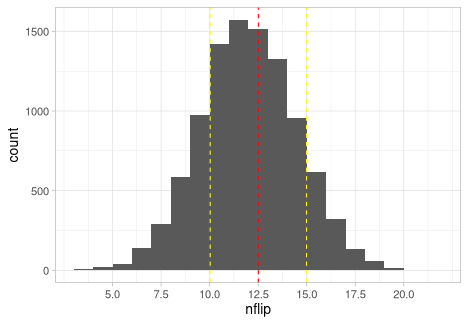
\includegraphics{05.pvalues_files/figure-latex/unnamed-chunk-2-1.png}

\begin{itemize}
\tightlist
\item
  Mean= 12.5101
\item
  Var = 6.1551135
\item
  SD = 2.4809501
\end{itemize}

\newpage

\hypertarget{ux441ux43fux43eux441ux442ux435ux440ux435ux436ux435ux43dux43dux44f}{%
\section{Спостереження}\label{ux441ux43fux43eux441ux442ux435ux440ux435ux436ux435ux43dux43dux44f}}

\begin{Shaded}
\begin{Highlighting}[]
\CommentTok{\# більш ніж 19}
\NormalTok{rare\_event }\OtherTok{\textless{}{-}} \DecValTok{19}
\FunctionTok{sum}\NormalTok{(binomial\_sim }\SpecialCharTok{\textgreater{}=}\NormalTok{ rare\_event) }\SpecialCharTok{/}\NormalTok{ bootstrap\_n}
\end{Highlighting}
\end{Shaded}

\begin{verbatim}
## [1] 0.008
\end{verbatim}

\begin{Shaded}
\begin{Highlighting}[]
\NormalTok{binomial\_sim}\SpecialCharTok{$}\NormalTok{nflip }\SpecialCharTok{\%\textgreater{}\%} \FunctionTok{table}\NormalTok{()}
\end{Highlighting}
\end{Shaded}

\begin{verbatim}
## .
##    3    4    5    6    7    8    9   10   11   12   13   14   15   16   17   18 
##    1    5   22   41  138  289  585  972 1419 1574 1517 1327  955  617  325  133 
##   19   20   21   22 
##   60   14    5    1
\end{verbatim}

\newpage

\hypertarget{p-ux437ux43dux430ux447ux435ux43dux43dux44f}{%
\section{P-значення}\label{p-ux437ux43dux430ux447ux435ux43dux43dux44f}}

\begin{Shaded}
\begin{Highlighting}[]
\FunctionTok{ggplot}\NormalTok{(binomial\_sim) }\SpecialCharTok{+} 
    \FunctionTok{geom\_histogram}\NormalTok{(}\FunctionTok{aes}\NormalTok{(}\AttributeTok{x =}\NormalTok{ nflip, }\AttributeTok{fill =}\NormalTok{ nflip }\SpecialCharTok{\textgreater{}=} \DecValTok{19}\NormalTok{), }\AttributeTok{binwidth =} \DecValTok{1}\NormalTok{, }\AttributeTok{boundary =} \DecValTok{5}\NormalTok{, }\AttributeTok{closed =} \StringTok{"left"}\NormalTok{) }\SpecialCharTok{+}
    \FunctionTok{geom\_vline}\NormalTok{(}\AttributeTok{xintercept =} \FunctionTok{mean}\NormalTok{(binomial\_sim}\SpecialCharTok{$}\NormalTok{nflip), }\AttributeTok{linetype =} \StringTok{"dashed"}\NormalTok{, }\AttributeTok{color =} \StringTok{"red"}\NormalTok{) }\SpecialCharTok{+}
    \FunctionTok{geom\_vline}\NormalTok{(}\AttributeTok{xintercept =} \FunctionTok{mean}\NormalTok{(binomial\_sim}\SpecialCharTok{$}\NormalTok{nflip) }\SpecialCharTok{+} \FunctionTok{sd}\NormalTok{(binomial\_sim}\SpecialCharTok{$}\NormalTok{nflip), }\AttributeTok{linetype =} \StringTok{"dashed"}\NormalTok{, }\AttributeTok{color =} \StringTok{"yellow"}\NormalTok{) }\SpecialCharTok{+}
    \FunctionTok{geom\_vline}\NormalTok{(}\AttributeTok{xintercept =} \FunctionTok{mean}\NormalTok{(binomial\_sim}\SpecialCharTok{$}\NormalTok{nflip) }\SpecialCharTok{{-}} \FunctionTok{sd}\NormalTok{(binomial\_sim}\SpecialCharTok{$}\NormalTok{nflip), }\AttributeTok{linetype =} \StringTok{"dashed"}\NormalTok{, }\AttributeTok{color =} \StringTok{"yellow"}\NormalTok{) }\SpecialCharTok{+}
    \FunctionTok{geom\_vline}\NormalTok{(}\AttributeTok{xintercept =} \DecValTok{19}\NormalTok{, }\AttributeTok{linetype =} \StringTok{"solid"}\NormalTok{, }\AttributeTok{color =} \StringTok{"black"}\NormalTok{) }\SpecialCharTok{+}
    \FunctionTok{scale\_x\_continuous}\NormalTok{(}\AttributeTok{breaks =} \FunctionTok{c}\NormalTok{(}\DecValTok{4}\NormalTok{, }\DecValTok{5}\NormalTok{, }\FloatTok{7.5}\NormalTok{, }\DecValTok{10}\NormalTok{, }\FloatTok{12.5}\NormalTok{, }\DecValTok{15}\NormalTok{, }\FloatTok{17.5}\NormalTok{, }\DecValTok{19}\NormalTok{, }\DecValTok{20}\NormalTok{), }
                       \AttributeTok{limits =} \FunctionTok{c}\NormalTok{(}\FunctionTok{min}\NormalTok{(binomial\_sim}\SpecialCharTok{$}\NormalTok{nflip), }\FunctionTok{max}\NormalTok{(binomial\_sim}\SpecialCharTok{$}\NormalTok{nflip))) }\SpecialCharTok{+} \FunctionTok{theme\_bw}\NormalTok{()}
\end{Highlighting}
\end{Shaded}

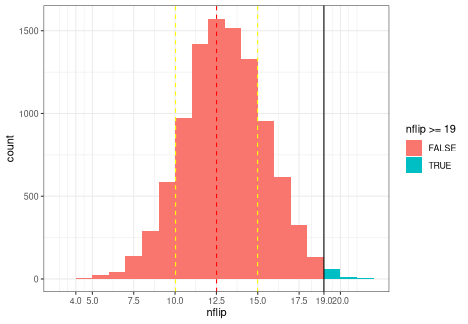
\includegraphics{05.pvalues_files/figure-latex/unnamed-chunk-5-1.png}

\begin{Shaded}
\begin{Highlighting}[]
\CommentTok{\#scale\_y\_log10()}
\end{Highlighting}
\end{Shaded}

\begin{itemize}
\tightlist
\item
  H0: монетка випадкова (p = 0.5) (нема біологічного сигнала)
\item
  тестова статистика: скільки успіхів (heads) із 25 експериментів
\item
  порахували розподіл ймовірності за методом Монте-Карло на 10,000
  повторів
\item
  оцінили, наскільки ймовірно, що H0 пояснює спостереження (більше 19)
\end{itemize}

\newpage

\hypertarget{nflip-15}{%
\section{nflip \textgreater= 15}\label{nflip-15}}

\begin{Shaded}
\begin{Highlighting}[]
\FunctionTok{ggplot}\NormalTok{(binomial\_sim) }\SpecialCharTok{+} 
    \FunctionTok{geom\_histogram}\NormalTok{(}\FunctionTok{aes}\NormalTok{(}\AttributeTok{x =}\NormalTok{ nflip, }\AttributeTok{fill =}\NormalTok{ nflip }\SpecialCharTok{\textgreater{}=} \DecValTok{15}\NormalTok{), }\AttributeTok{binwidth =} \DecValTok{1}\NormalTok{, }\AttributeTok{boundary =} \DecValTok{5}\NormalTok{, }\AttributeTok{closed =} \StringTok{"left"}\NormalTok{) }\SpecialCharTok{+}
    \FunctionTok{geom\_vline}\NormalTok{(}\AttributeTok{xintercept =} \FunctionTok{mean}\NormalTok{(binomial\_sim}\SpecialCharTok{$}\NormalTok{nflip), }\AttributeTok{linetype =} \StringTok{"dashed"}\NormalTok{, }\AttributeTok{color =} \StringTok{"red"}\NormalTok{) }\SpecialCharTok{+}
    \FunctionTok{geom\_vline}\NormalTok{(}\AttributeTok{xintercept =} \FunctionTok{mean}\NormalTok{(binomial\_sim}\SpecialCharTok{$}\NormalTok{nflip) }\SpecialCharTok{+} \FunctionTok{sd}\NormalTok{(binomial\_sim}\SpecialCharTok{$}\NormalTok{nflip), }\AttributeTok{linetype =} \StringTok{"dashed"}\NormalTok{, }\AttributeTok{color =} \StringTok{"yellow"}\NormalTok{) }\SpecialCharTok{+}
    \FunctionTok{geom\_vline}\NormalTok{(}\AttributeTok{xintercept =} \FunctionTok{mean}\NormalTok{(binomial\_sim}\SpecialCharTok{$}\NormalTok{nflip) }\SpecialCharTok{{-}} \FunctionTok{sd}\NormalTok{(binomial\_sim}\SpecialCharTok{$}\NormalTok{nflip), }\AttributeTok{linetype =} \StringTok{"dashed"}\NormalTok{, }\AttributeTok{color =} \StringTok{"yellow"}\NormalTok{) }\SpecialCharTok{+}
    \FunctionTok{geom\_vline}\NormalTok{(}\AttributeTok{xintercept =} \DecValTok{15}\NormalTok{, }\AttributeTok{linetype =} \StringTok{"solid"}\NormalTok{, }\AttributeTok{color =} \StringTok{"black"}\NormalTok{) }\SpecialCharTok{+}
    \FunctionTok{scale\_x\_continuous}\NormalTok{(}\AttributeTok{breaks =} \FunctionTok{c}\NormalTok{(}\DecValTok{4}\NormalTok{, }\DecValTok{5}\NormalTok{, }\FloatTok{7.5}\NormalTok{, }\DecValTok{10}\NormalTok{, }\FloatTok{12.5}\NormalTok{, }\DecValTok{15}\NormalTok{, }\FloatTok{17.5}\NormalTok{, }\DecValTok{19}\NormalTok{, }\DecValTok{20}\NormalTok{), }
                       \AttributeTok{limits =} \FunctionTok{c}\NormalTok{(}\FunctionTok{min}\NormalTok{(binomial\_sim}\SpecialCharTok{$}\NormalTok{nflip), }\FunctionTok{max}\NormalTok{(binomial\_sim}\SpecialCharTok{$}\NormalTok{nflip))) }\SpecialCharTok{+} \FunctionTok{theme\_bw}\NormalTok{()}
\end{Highlighting}
\end{Shaded}

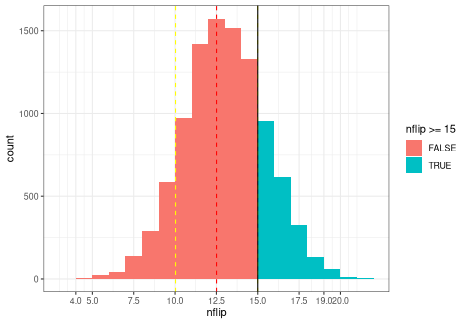
\includegraphics{05.pvalues_files/figure-latex/unnamed-chunk-6-1.png}

\begin{Shaded}
\begin{Highlighting}[]
\NormalTok{rare\_event }\OtherTok{\textless{}{-}} \DecValTok{15}
\FunctionTok{sum}\NormalTok{(binomial\_sim }\SpecialCharTok{\textgreater{}=}\NormalTok{ rare\_event) }\SpecialCharTok{/}\NormalTok{ bootstrap\_n}
\end{Highlighting}
\end{Shaded}

\begin{verbatim}
## [1] 0.211
\end{verbatim}

\newpage

\hypertarget{ux43aux43bux430ux441ux442ux435ux440-ux445ux432ux43eux440ux43eux431ux438}{%
\section{Кластер
хвороби}\label{ux43aux43bux430ux441ux442ux435ux440-ux445ux432ux43eux440ux43eux431ux438}}

\begin{itemize}
\item
  \textless{} 10 км від атомної станції: 5.8 випадків на 10,000: 47 /
  80,515
\item
  \(>\) 30 км від атомної станції: 4.7 випадків на 10,000: 851 /
  1,819,636
\item
  incidence ratio: 5.8/4.7 = 1.23
\item
  H0: IR = 4.7
\item
  тестова статистика: кількість захворювань \%
\item
  розподіл тестової статистики за припущення H0
\end{itemize}

\begin{Shaded}
\begin{Highlighting}[]
\NormalTok{sim\_cancer }\OtherTok{\textless{}{-}} \FunctionTok{do}\NormalTok{(}\DecValTok{10000}\NormalTok{)}\SpecialCharTok{*}\FunctionTok{nflip}\NormalTok{(}\AttributeTok{n =} \DecValTok{80515}\NormalTok{, }\AttributeTok{prob =} \FloatTok{0.00047}\NormalTok{)}
\FunctionTok{ggplot}\NormalTok{(sim\_cancer) }\SpecialCharTok{+} 
  \FunctionTok{geom\_histogram}\NormalTok{(}\FunctionTok{aes}\NormalTok{(}\AttributeTok{x =}\NormalTok{ nflip), }\AttributeTok{binwidth =} \DecValTok{1}\NormalTok{)}
\end{Highlighting}
\end{Shaded}

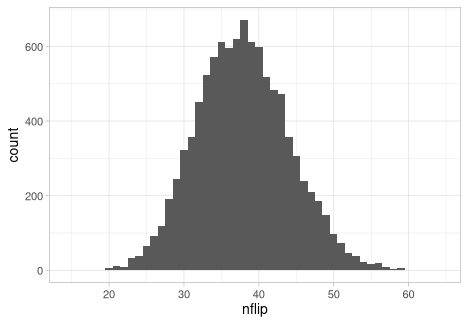
\includegraphics{05.pvalues_files/figure-latex/unnamed-chunk-8-1.png}

\begin{itemize}
\tightlist
\item
  Mean= 37.8623
\item
  Var = 37.9789366
\item
  SD = 6.1627053
\item
  P = 0.0874
\end{itemize}

\newpage

\begin{Shaded}
\begin{Highlighting}[]
\FunctionTok{ggplot}\NormalTok{(sim\_cancer) }\SpecialCharTok{+} 
    \FunctionTok{geom\_histogram}\NormalTok{(}\FunctionTok{aes}\NormalTok{(}\AttributeTok{x =}\NormalTok{ nflip, }\AttributeTok{fill =}\NormalTok{ nflip }\SpecialCharTok{\textgreater{}=} \DecValTok{47}\NormalTok{), }\AttributeTok{binwidth =} \DecValTok{1}\NormalTok{, }\AttributeTok{boundary =} \DecValTok{5}\NormalTok{, }\AttributeTok{closed =} \StringTok{"left"}\NormalTok{) }\SpecialCharTok{+}
    \FunctionTok{geom\_vline}\NormalTok{(}\AttributeTok{xintercept =} \FunctionTok{mean}\NormalTok{(sim\_cancer}\SpecialCharTok{$}\NormalTok{nflip), }\AttributeTok{linetype =} \StringTok{"dashed"}\NormalTok{, }\AttributeTok{color =} \StringTok{"red"}\NormalTok{) }\SpecialCharTok{+}
    \FunctionTok{geom\_vline}\NormalTok{(}\AttributeTok{xintercept =} \FunctionTok{mean}\NormalTok{(sim\_cancer}\SpecialCharTok{$}\NormalTok{nflip) }\SpecialCharTok{+} \FunctionTok{sd}\NormalTok{(sim\_cancer}\SpecialCharTok{$}\NormalTok{nflip), }\AttributeTok{linetype =} \StringTok{"dashed"}\NormalTok{, }\AttributeTok{color =} \StringTok{"yellow"}\NormalTok{) }\SpecialCharTok{+}
    \FunctionTok{geom\_vline}\NormalTok{(}\AttributeTok{xintercept =} \FunctionTok{mean}\NormalTok{(sim\_cancer}\SpecialCharTok{$}\NormalTok{nflip) }\SpecialCharTok{{-}} \FunctionTok{sd}\NormalTok{(sim\_cancer}\SpecialCharTok{$}\NormalTok{nflip), }\AttributeTok{linetype =} \StringTok{"dashed"}\NormalTok{, }\AttributeTok{color =} \StringTok{"yellow"}\NormalTok{) }\SpecialCharTok{+}
    \FunctionTok{geom\_vline}\NormalTok{(}\AttributeTok{xintercept =} \DecValTok{47}\NormalTok{, }\AttributeTok{linetype =} \StringTok{"solid"}\NormalTok{, }\AttributeTok{color =} \StringTok{"black"}\NormalTok{) }\SpecialCharTok{+}
    \FunctionTok{scale\_x\_continuous}\NormalTok{(}\AttributeTok{breaks =} \FunctionTok{c}\NormalTok{(}\DecValTok{25}\NormalTok{, }\DecValTok{32}\NormalTok{, }\DecValTok{38}\NormalTok{, }\DecValTok{44}\NormalTok{, }\DecValTok{50}\NormalTok{), }
                       \AttributeTok{limits =} \FunctionTok{c}\NormalTok{(}\FunctionTok{min}\NormalTok{(sim\_cancer}\SpecialCharTok{$}\NormalTok{nflip), }\FunctionTok{max}\NormalTok{(sim\_cancer}\SpecialCharTok{$}\NormalTok{nflip))) }\SpecialCharTok{+} \FunctionTok{theme\_bw}\NormalTok{()}
\end{Highlighting}
\end{Shaded}

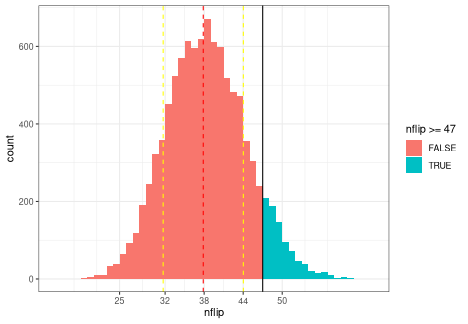
\includegraphics{05.pvalues_files/figure-latex/unnamed-chunk-9-1.png}

\newpage

\hypertarget{sessioninfo}{%
\section{sessionInfo()}\label{sessioninfo}}

\begin{Shaded}
\begin{Highlighting}[]
\FunctionTok{sessionInfo}\NormalTok{()}
\end{Highlighting}
\end{Shaded}

\begin{verbatim}
## R version 4.4.1 (2024-06-14)
## Platform: x86_64-redhat-linux-gnu
## Running under: Fedora Linux 40 (Workstation Edition)
## 
## Matrix products: default
## BLAS/LAPACK: FlexiBLAS OPENBLAS-OPENMP;  LAPACK version 3.11.0
## 
## locale:
##  [1] LC_CTYPE=en_US.UTF-8       LC_NUMERIC=C              
##  [3] LC_TIME=en_US.UTF-8        LC_COLLATE=en_US.UTF-8    
##  [5] LC_MONETARY=en_US.UTF-8    LC_MESSAGES=en_US.UTF-8   
##  [7] LC_PAPER=en_US.UTF-8       LC_NAME=C                 
##  [9] LC_ADDRESS=C               LC_TELEPHONE=C            
## [11] LC_MEASUREMENT=en_US.UTF-8 LC_IDENTIFICATION=C       
## 
## time zone: America/Toronto
## tzcode source: system (glibc)
## 
## attached base packages:
## [1] stats     graphics  grDevices utils     datasets  methods   base     
## 
## other attached packages:
##  [1] knitr_1.48        mosaic_1.9.1      mosaicData_0.20.4 ggformula_0.12.0 
##  [5] Matrix_1.7-0      lattice_0.22-6    lubridate_1.9.3   forcats_1.0.0    
##  [9] stringr_1.5.1     dplyr_1.1.4       purrr_1.0.2       readr_2.1.5      
## [13] tidyr_1.3.1       tibble_3.2.1      ggplot2_3.5.1     tidyverse_2.0.0  
## 
## loaded via a namespace (and not attached):
##  [1] utf8_1.2.4         generics_0.1.3     stringi_1.8.4      hms_1.1.3         
##  [5] digest_0.6.36      magrittr_2.0.3     evaluate_0.24.0    grid_4.4.1        
##  [9] timechange_0.3.0   fastmap_1.2.0      fansi_1.0.6        scales_1.3.0      
## [13] cli_3.6.3          labelled_2.13.0    rlang_1.1.4        munsell_0.5.1     
## [17] withr_3.0.0        yaml_2.3.9         tools_4.4.1        tzdb_0.4.0        
## [21] colorspace_2.1-0   mosaicCore_0.9.4.0 vctrs_0.6.5        R6_2.5.1          
## [25] ggridges_0.5.6     lifecycle_1.0.4    MASS_7.3-60.2      pkgconfig_2.0.3   
## [29] pillar_1.9.0       gtable_0.3.5       glue_1.7.0         highr_0.11        
## [33] haven_2.5.4        xfun_0.45          tidyselect_1.2.1   rstudioapi_0.16.0 
## [37] farver_2.1.2       htmltools_0.5.8.1  labeling_0.4.3     rmarkdown_2.27    
## [41] compiler_4.4.1
\end{verbatim}

\end{document}
